\def\year{2018}\relax
%File: formatting-instruction.tex
\documentclass[letterpaper]{article} %DO NOT CHANGE THIS
\usepackage{aaai18}  %Required
\usepackage{times}  %Required
\usepackage{helvet}  %Required
\usepackage{courier}  %Required
\usepackage{url}  %Required
\usepackage{graphicx}  %Required
\frenchspacing  %Required
\setlength{\pdfpagewidth}{8.5in}  %Required
\setlength{\pdfpageheight}{11in}  %Required
%\copyrighttext{Copyright 2017. All rights reserved.}
%PDF Info Is Required:
  \pdfinfo{
%/Title (Extracting Information from Scientific Publications for
%Planetary Science)
/Title (Mars Target Encyclopedia: Rock and Soil Composition Extracted
from the Literature)
/Author (Kiri L. Wagstaff, Raymond Francis, Thamme Gowda, Nina L. Lanza,
You Lu, Ellen Riloff, Karanjeet Singh)}
\setcounter{secnumdepth}{0}  
 \begin{document}
% The file aaai.sty is the style file for AAAI Press 
% proceedings, working notes, and technical reports.
%
%\title{Extracting Information from Scientific Publications for
%Planetary Science}
\title{Mars Target Encyclopedia: \\ Rock and Soil Composition Extracted
from the Literature}
\author{
Kiri L. Wagstaff$^1$,
Raymond Francis$^1$,
Thamme Gowda$^{1,2}$,
You Lu$^1$,\\
{\Large \bf 
Ellen Riloff$^3$, 
Karanjeet Singh$^1$, and
Nina L. Lanza$^4$}\\
$^1$Jet Propulsion Laboratory, California Institute of Technology,
%4800 Oak Grove Drive, 
Pasadena, CA 91109, \{firstname.lastname\}@jpl.nasa.gov\\
$^2$Information Sciences Institute, University of Southern
California,
%4676 Admiralty Way \#1001, 
Marina Del Rey, CA 90292, tg@isi.edu\\
$^3$School of Computing, University of Utah,
%50 S. Central Campus Drive, 
Salt Lake City, UT 84112, riloff@cs.utah.edu\\
$^4$Los Alamos National Laboratory, Los Alamos, NM 87545,
nlanza@lanl.gov\\
}
\maketitle
\begin{abstract}
We have constructed an information extraction system called the Mars
Target Encyclopedia that takes in planetary science publications
and extracts scientific knowledge about target compositions.
The extracted knowledge is stored in a searchable database that can
greatly accelerate the ability of scientists to compare new
discoveries with what is already known.  To date, we have applied this
system to $\sim$6000 documents and achieved 50--64\% precision in the
extracted information.  
\end{abstract}
% lpsc14: 1908
% lpsc15: 1991
% lpsc16: 2060
% total: 5959

\section{Introduction}

Scientists everywhere are overwhelmed by the stream of new information
that is published by their disciplines' conferences, workshops, and
journals.  It is increasingly difficult to come up to speed in a
new area and to stay current with the latest discoveries.  In
planetary exploration, new discoveries can occur each time
new data is transmitted.  For example, our rovers on Mars have sent
back compositional data for thousands of individual targets (e.g.,
rocks, soils), and some of those observations have transformed our
understanding of past environments on the
planet~\cite{grotzinger:ykb14}. 

To interpret new observations correctly, it is necessary to be able to
compare them with what is already known.  For example, if we observe
high manganese content at a particular location, we want to know
whether it is consistent with previous observations or it indicates an
anomalous new discovery.  However, no central database exists in which
planetary scientists can quickly make that determination.

We have created a system called the Mars Target Encyclopedia (MTE)
that uses information extraction methods to analyze planetary science
publications and identify stated compositional relationships between Mars
surface targets and elements or minerals.  The extracted information
is stored in a searchable database that allows users to ask questions
such as ``Which targets contain hematite?'' or ``What is known about
target Dillinger?''  It also enables entirely new kinds of information
visualization, such as a map display of all locations where the Mars
rover Curiosity has detected hematite.  Ultimately, the MTE may serve 
as a resource to inform
%the development of hypotheses about the history and evolution of Mars
%surface processes as well as 
decisions about the next steps in Mars exploration.  

%leveraged a small amount of hand-labeled text to train a

In this paper, we describe the MTE system and its component
technologies, the empirical performance of the system on labeled data,
and results from a large-scale evaluation on $\sim$6000 documents.
The MTE is currently being integrated into a public website called the
PDS (Planetary Data System) Analyst's Notebook for Mars scientists
and the public to access.  The automated pipeline can be used to
ingest and analyze new publications as they become available.

%precision more important than recall

\section{Related Work}

A variety of text analysis methods exist for extracting information
from text.  Some methods focus on extracting meta-data such as the
document title, authors, and publication venue or analyzing and
linking citations between papers~\cite{ronzano:scipub16}.
%
However, understanding the content of a scientific publication
requires a deeper analysis.  Information extraction (IE) of this
nature is generally broken into two steps: (1) named entity
recognition, to identify references to people, locations, and other
objects of interest, and (2) relation extraction, to identify
relationships between pairs of entities~\cite{mooney:ie05}.  Many of
the recent advances in IE have been motivated by problems from the
biomedical research world, such as the desire to identify
protein-protein interactions~\cite{tikk:protein10,bui:protein11} or
%\citeauthor{krallinger:chemistry17} (\citeyear{krallinger:chemistry17})
%provide an in-depth review of methods for recognizing chemical
%entities and identifying 
chemical-protein and chemical-disease
relations~\cite{krallinger:chemistry17}.  \citeauthor{tsutsui:ad16}
(\citeyear{tsutsui:ad16}) used topic modeling and open IE, which does
not require the prior identification of entities, to build a knowledge
database about Alzheimer's disease.
%Others have developed systems to extract information about the
%experiments conducted in machine translation papers~\cite{choi:mt16} 

To date, little such work has been done in the domain of planetary
science. The closest existing work is the geology-based GeoDeepDive
project, which performs text data mining on scientific publications
about (Earth) rock formations and
stratigraphy~\cite{zhang:geodeepdive13}.
% see also https://geodeepdive.org/about.html
% where they seem to have expanded - the language at least is
% not just about Geo.  But DeepDive itself is the generic version,
% I think?
%
%- other work at ISI, etc.  Can't find any!!!  Not even for geology.
% PaleoDeepDive is the closest and that's fossils.
By applying and extending information extraction methods to planetary
science publications, we have the opportunity to benefit an entirely
new population of scientists, researchers, and interested members of
the public.

\section{Machine Learning for Information Extraction}

The Mars Target Encyclopedia (MTE) is an information extraction system
that takes in scientific publications in PDF format and extracts
knowledge that is useful to scientists studying the planet Mars.
%
We focus on the extraction of information about targets (e.g., rocks,
soils) identified by the ChemCam instrument on the Curiosity rover.
ChemCam uses a laser spectrometer to obtain compositional spectra from
up to seven meters away from a given target. The resulting spectra can
be analyzed to identify individual elements within the
target~\cite{maurice:chemcam12}.  As of sol 1159 of the Curiosity
rover's mission, ChemCam had observed more than 1100 distinct targets.
New discoveries about these targets are published in a variety of
planetary science conference and journal venues.

The MTE is composed of four modules: preprocessing, named entity
recognition (NER), relation extraction (RE), and database updates (see
Figure~\ref{fig:mte}).

\begin{figure}
\begin{center}
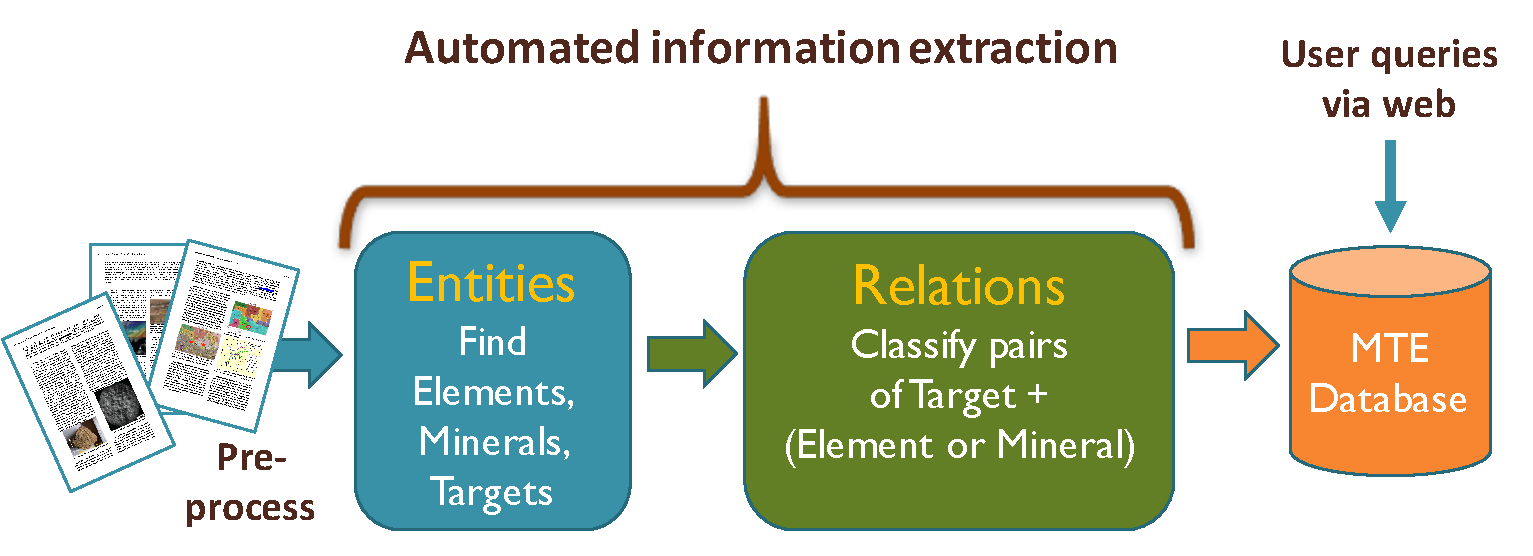
\includegraphics[width=3.25in]{fig/system.pdf}
\end{center}
\caption{Mars Target Encyclopedia processing pipeline.}
\label{fig:mte}
\end{figure}
% This figure comes from 2017-06-23-mte.pptx

\subsection{Document Preprocessing}

To prepare the documents for information extraction, the MTE first
extracts the text content from each PDF document.  We use the Apache
Tika parser~\cite{mattmann:tika11} to convert the source PDF files
into UTF-8 format text to preserve accented characters and
mathematical symbols.
% more details from extract_text_utf8.py?
Next, the MTE creates a copy of the text content in which the
References section is omitted.  We defined a regular expression to
identify the References section.
% show the regexp?
This step helps the NER module avoid spurious detections in the
titles or author names of cited publications.

\subsection{Named Entity Recognition}

The named entities of greatest relevance for the MTE are elements
(e.g., ``iron,'' ``Mg''), minerals (e.g., ``plagioclase,''
``hematite''), and ChemCam targets.  The periodic table provides a
comprehensive list of elements, and we employed a list of 5228
minerals provided by the International Mineralogical Association (the
May 2017 release\footnote{\url{http://nrmima.nrm.se/imalist.htm}}). 

Identifying Mars surface targets is more challenging, as they follow
no standard naming convention.  Further, target names are
fundamentally ambiguous as they are borrowed from Earth locations or
people.  A sampling of the names hints at the challenge of accurately
detecting them: ``Dunkirk'', ``Ithaca'', ``Jake'', ``Old\_woman'',
``Pistol''.  We have a starting list of target
names\footnote{\url{http://pds-geosciences.wustl.edu/msl/msl-m-chemcam-libs-4_5-rdr-v1/mslccm_1xxx/document/msl_ccam_obs.csv}}
that was published by the ChemCam science team, but it is not fully
curated, and we have found it to be incomplete with respect to the
literature.
%
In addition, we found that authors continually invent new spelling
variants and abbreviations for target names that require more than a
simple list lookup.
% Keyword-based web or publication searches return many spurious hits.

To address the challenge of recognizing all three entity classes
reliably, we employed a machine learning approach.  We trained a
custom Named Entity Recognizer using the Stanford CoreNLP NER
system~\cite{finkel:ner05}.  This system trains a Conditional Random
Field sequence model to assign class labels to entities within new
documents.  We provided manually labeled documents with examples of
the Element, Mineral, and Target classes to train our custom
model.  We also employed the ``gazette'' capability to provide lists
of known terms.  This is particularly valuable for large semantic
classes (like Mineral or Target) in which terms exist that might never
appear in the training corpus.  The gazettes that we used include the
periodic table (Elements), the IMA list (Minerals), and the ChemCam
observation table (Targets) as mentioned above.

%{\bf Steven: add paragraph describing details of converting our text and
%annotations into CoreNLP data format (inside/outside encoding).}

% TODO:
%{\bf [gazettes are available where online]}

%% We also employed the Basilisk bootstrapping algorithm to learn
%% additional related terms that belong to each entity
%% class~\cite{thelen:basilisk02}.  {\bf [Ellen: add brief blurb about
%% Basilisk]}  It was our hope that Basilisk, which operates on unlabeled
%% text, might learn terms that would otherwise escape the CRF
%% classifier, which can only learn from labeled text.  These could
%% include author-created abbreviations and alternate spellings.

% Ellen's Basilisk text

%% Another challenge of real-world text processing is the prevalence of
%% non-standard terms that are variants or edge cases of an entity
%% type. For example, planetary science articles often mention not only
%% individual Elements but combinations of Elements (e.g., ``U-Th'' or
%% ``Zr/Si''), specific isotopes (e.g., ``47Ti''), categories of elements
%% (e.g., ``alkalis''), abbreviations (e.g., ``REEs'' for Rare Earth
%% Elements), and spelling variants (e.g., ``alkalies''). To enhance our
%% ability to recognize non-standard vocabulary, we employed the Basilisk
%% bootstrapping algorithm for semantic lexicon induction
%% \cite{thelen:basilisk02}. Basilisk automatically generates lexical
%% dictionaries using a small set of ``seed'' words for each semantic
%% category to be learned, and a large collection of raw texts for the
%% targeted domain. Basilisk iteratively grows the dictionaries by
%% discovering lexico-syntactic patterns that consistently co-occur with
%% the seed words and then using the patterns to hypothesize new category
%% members, which are added to the dictionary and serve as new seed
%% words for bootstrapped learning.  It was our hope that Basilisk, which
%% can learn from unannotated documents, might learn additional
%% terminology that would otherwise escape the CRF classifier, which can
%% only learn from manually annotated documents.

%% We applied Basilisk to X documents from LPSC 2014 and LPSC 2015.  We
%% used Basilisk to generate lexicons for six semantic categories: {\it
%%  Elements, Instruments, Locations, Minerals, Spacecraft,} and {\it
%%  Targets}. Although we did not need instruments, locations, or
%% spacecraft for the MTE, we found that these entities often appeared in
%% contexts similar to those surrounding elements, minerals, and targets,
%% so Basilisk benefits from learning to distinguish these ``negative''
%% categories too. As input, we provided Basilisk with the following seed
%% word lists: ....

\subsection{Relation Extraction}

Once the entities are identified within the text, the MTE analyzes them
to determine which ones have a compositional relationship (i.e.,
textual evidence that a given Target contains a given Element or
Mineral).  
%
We trained a relation classifier using the jSRE~\cite{giuliano:jsre06}
relation extraction tool.  It uses an SVM classifier to predict
whether a relationship exists for two entities, using only shallow
parsing.  jSRE provides SVM kernels that operate on local context,
global (sentence-wide) context, or a combination of both.  In applying
this method to biomedical publications, the authors found that most of
the performance came from the global kernel features.

% TODO
%{\bf Kiri: add details about jSRE example format encoding;
%multi-word tokens should be merged with underscores... instead, we
%operated on a per-word basis and merged relations as appropriate (hack)}

\subsection{MTE Database}

For each document, the MTE database stores document meta-data (e.g.,
title, author, publication venue), the preprocessed text content, and
the extracted entities and relations.  To provide full traceability,
it also stores the parsed sentence from which the relation was
extracted and a link to the original PDF.  Users can immediately see
the source context and decide whether they would like to access the
full document for more information.
 
To support fast retrieval of
documents that contain entities or relations specified in a given
search queries, we constructed inverted indices for the entities and
relations using Apache
Solr\footnote{\url{http://lucene.apache.org/solr/}}. Apache Solr is an
open source search platform powered by Apache Lucene that provides
near real-time search and document retrieval. 
%The storing of content was accomplished by a program that was at the
%end of MTE pipeline described in Figure {\ref fig1}. The querying
%functionality was offered as an API to the MTE web interface, the
%discussion of it is beyond the scope of this article {\cite
%https://www.hou.usra.edu/meetings/planetdata2017/pdf/7031.pdf}
 
\section{Experimental Results}

We developed and evaluated the MTE using a collection of scientific
papers that were published over three years of the Lunar and Planetary
Science Conference (LPSC).  These papers are publicly accessible from
the LPSC websites
(e.g., \url{https://www.hou.usra.edu/meetings/lpsc2014/}). 

\subsection{Corpus}

Our corpus consists of two-page extended LPSC abstracts in PDF format.
We selected 117 documents from LPSC 2015 and 2016 that mentioned
``ChemCam.''  We used the html-based brat annotation tool~\cite{brat}
to manually label entities and relations within these documents.  We
estimate that it took an average of 30 minutes to annotate each
document, or a total of more than 58 hours of labor for the full
corpus.  We created thousands of manual
annotations~\cite{francis:mte-data} in 62 documents from LPSC 2015 and
55 documents from LPSC 2016 (see Table~\ref{tab:docs}).

% cut -f2 *.ann | cut -f1 -d' ' | cut -f1 -d':' | sort | uniq -c
\begin{table}
\caption{Manual annotations for LPSC documents.}
\label{tab:docs}
\begin{center}
\begin{tabular}{l|ccc}
           & 2015     & 2016     & Total \\ 
Annotation & (62 docs) & (55 docs) & (117 docs)\\ \hline
Element  & 1195 & 1029 & 2224 \\
Mineral  & 748  & 708  & 1456 \\
Target   & 566  & 347  &  913 \\ \hline
Contains & 434  & 262  &  696 \\ \hline
Total    & 2943 & 2346 & 5289 \\ \hline
\end{tabular}
\end{center}
\end{table}

The annotated relationships ranged from simple (e.g., a pattern such
as ``X contains Y'' within a sentence) to complex (e.g., relationships
that crossed sentence boundaries or involved pronouns like ``it'' and
other anaphora).  Figure~\ref{fig:brat} shows an excerpt from one
document that contains several statements about the composition of the
target Big Sky.  The vocabulary used to indicate a compositional
relationship varies, and the final relationship crosses a sentence
boundaries.  

% lpsc16-1155
\begin{figure}
\begin{center}
%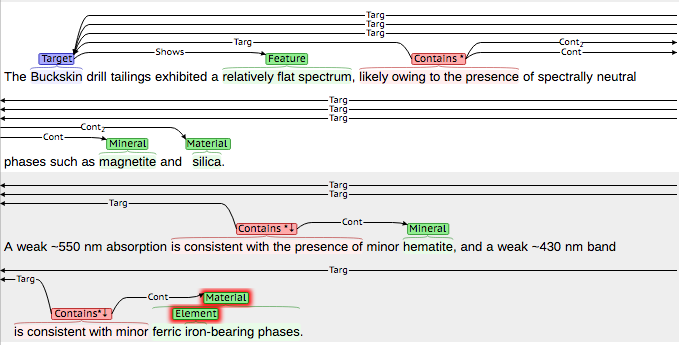
\includegraphics[width=3.25in]{fig/brat-example.png}
%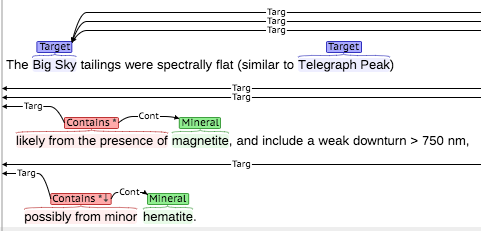
\includegraphics[width=3.25in]{fig/lpsc16-1155-bigsky.png}
\includegraphics[width=3.25in]{fig/lpsc16-1155-bigsky-2.png}
\end{center}
\caption{Excerpt from document lpsc16-1155 showing compositional
annotations created with the brat web annotation tool.}
\label{fig:brat}
\end{figure}

% TODO:
%{\bf [annotated docs are available where?]}

\subsection{Named Entity Recognition Results}

Named entity recognition operates on individual words or tokens.  We
used the 2015 documents for training and divided the 2016 documents
into validation ($n=20$) and testing ($n=35$) sets.  
%(Total number of items?) 
Training a basic NER classifier using the CoreNLP system yielded an
F1-score of 0.805.  Precision was very high (nearly 0.95), and recall
was 0.70.  Recall was highest (0.84) for the Element class, as
expected; it was 0.73 for Minerals and 0.28 for Targets.  The Target
class is the most difficult one to recognize due to the lack of a
naming convention and ambiguous names.  In addition, the Target class
grows much faster than the set of known elements or minerals, so there
will always be new targets in future documents that never appeared in
the training set.

However, we were able to improve NER recall by including the gazettes
as described above.  These term lists augment the manually labeled
documents and provide relevant domain knowledge.  With the gazettes,
F1-score increased to 0.853 by boosting recall to 0.777.  Recall for
the Target class, in particular, more than doubled, to 0.67.

\begin{table}
\caption{Named entity recognition performance on LPSC 2016 test documents.  
The best result is shown in bold.}
\label{tab:ner}
\begin{center}
\begin{tabular}{l|ccc}
 & Prec. & Recall & F1 \\ \hline
%Baseline: Lists only & 0.592 & 0.867 & 0.703 \\ \hline  % all LPSC16
Baseline: Lists only & 0.831 & 0.699 & 0.760 \\ \hline  % LPSC16-test
% TODO: resolve the fact that I get different numbers for the 
% rows below when running my eval_brat script (which is how I got
% the baseline numbers above).  Otherwise not a fair comparison.
{\em CoreNLP NER CRF trained on:} & & \\
% Numbers reported by Steven (CoreNLP)
LPSC 2015            & {\bf 0.948} & 0.700 & 0.805 \\
LPSC 2015 + gazettes & 0.945 & {\bf 0.777} & {\bf 0.853} \\
%LPSC 2015 + Basilisk gazettes & P & R \\
\hline
\end{tabular}
\end{center}
\end{table}

%{\bf [precision/recall per class - bar plot?]}

% TODO
%Basilisk - output manually reviewed

\subsection{Relation Extraction Results}

The decision about whether or not a relation exists is made for a
given pair of entities.  Processing all possible pairs of entities in
a document would be infeasible (and likely unnecessary).  For
simplicity, we adopted the strategy used in previous
work~\cite{giuliano:jsre06} of generating all pairs of entities that
occur within a single sentence.  We used CoreNLP's sentence splitter
to divide the corpus into sentences and the NER model trained above to
identify entities.  For each (Target, Element) or (Target, Mineral)
pair, we generated a jSRE example that encoded the sentence content.
If the pair of entities was connected by a relation in the manual
annotations, we gave the example a positive label; otherwise, we gave
it a negative label.

To simulate how the system would be used in practice, we trained and
validated the relation classifier using text from LPSC 2015 and tested
it on LPSC 2016.  We used the first 42 LPSC 2015 documents for
training and the remaining 20 for validation.  The number and
distribution of the resulting jSRE examples (relationships) are given
in Table~\ref{tab:rels}.  

% for l in lpsc16-utf8/*test ; do echo $l ; cut -f1 $l | sort | uniq -c; done
\begin{table}[b]
\caption{Number and distribution of relationships between Targets and
Elements or Minerals. The number in parentheses is the percentage of
positive relationships. }
\label{tab:rels}
\begin{center}
\begin{tabular}{l|ccc}
           & Element & Mineral & Merged \\ \hline 
Train      & 279 (38\%) & 150 (41\%) & 429 (39\%) \\
Validation &  93 (27\%) &  70 (69\%) & 163 (45\%) \\ \hline
Test       & 111 (37\%) &  62 (50\%) & 173 (42\%) \\ \hline
\end{tabular}
\end{center}
\end{table}

We trained three different relation classifiers: one on Target-Element
relations only; one on Target-Mineral relations only; and one on the
merged set.  We were curious as to how a specialized model that was
trained on less data would compare to a more generic model trained on
more data.  For each model, we performed a grid search over the jSRE
parameters by trying each of the SVM kernels (LC, GC, SL) and window
sizes within the set \{ 1, 2, 5, 10, 15, 20 \}.  We selected the model
parameters that led to the highest performance on the validation set
in terms of precision.  We found that the max-precision model did not
employ the same parameters across the three models.  jSRE-Elements and
jSRE-Merged used an LC kernel with a window of 5, while jSRE-Minerals
used an SL kernel with a window of 5.  Notably, the GC kernel that the
original authors found to be most powerful for the biomedical domain
did not perform well in this corpus.

We found that the individual models (jSRE-Elements and jSRE-Minerals)
achieved much higher precision than a baseline approach that always
predicted that a relationship was present (``All-yes'') (see
Table~\ref{tab:re}).  While this baseline always achieves a recall of
1.00 and therefore appears superior in terms of F-measure, this
application domain values precision much more than recall.  Content
included in the MTE must be of the highest reliability, even if
this means it is not comprehensive.  
%
We also found that the merged model (jSRE-Merged) out-performed the
baseline and the individual models when they were applied to the full
(Merged) data set (jSRE-Indiv.). 

% TODO: add comparison to OpenIE

\begin{table}
\caption{Relation extraction performance on LPSC 2016 (test) documents. 
The highest-precision result for each data set is shown in bold.}
\label{tab:re}
\begin{center}
\begin{tabular}{l|ccc}
 & Precision & Recall & F1 \\ \hline
%{\em jSRE SVM trained on:} & & \\
\multicolumn{4}{c}{Elements ($n=111$)} \\
Baseline: All-yes & 0.369 & {\bf 1.000} & {\bf 0.539} \\ 
jSRE-Elements & {\bf 0.531} & 0.415 & 0.466 \\ \hline
\multicolumn{4}{c}{Minerals ($n=62$)} \\
Baseline: All-yes & 0.500 & {\bf 1.000} & {\bf 0.667} \\ 
jSRE-Minerals & {\bf 0.679} & 0.613 & 0.644 \\ \hline 
\multicolumn{4}{c}{Merged ($n=173$)} \\
Baseline: All-yes & 0.416 & {\bf 1.000} & {\bf 0.588} \\ 
jSRE-Indiv.  & 0.598 & 0.447 & 0.511 \\
jSRE-Merged  & {\bf 0.640} & 0.444 & 0.525 \\ \hline
\end{tabular}
\end{center}
\end{table}

%Also:
%- mineral is an easier problem than element?
%- these are separate evaluations because separate data sets
%- recall is somewhat low, but precision is far more important

\subsection{Large-scale Evaluation}

We collected all LPSC documents that were published in 2014, 2015, and
2016 ($n=5959$) and ingested them into the MTE.  This large corpus
contains the 117 documents used for development and evaluation as well
as everything else that was published at these conferences.

% TODO
%{\bf [table of num docs, num NER, num RE, time consumed]}

It would be infeasible to ask humans to manually label all 5959
documents to evaluate our results, so instead we performed a manual
review of only the extracted relations.  This allows us to measure
precision, but not recall.  However, as noted above, precision is far more
important than recall in this domain, as it captures the true utility
of the extracted information when used in practice.
%: it is vital that any information stored in the
%MTE is reliable and correct, even if it is incomplete.

The manual review results are shown in Table~\ref{tab:large}.  Our
manual reviewer examined each extracted relation and its source
sentence to judge the relation as Correct, Partial (e.g., only one
word of a multi-word Target name was extracted), Irrelevant (a correct
extraction from the sentence, but the content was not about Mars),
Wrong, or Unsure (the reviewer could not determine whether the
relation was correct).
% Add examples of each category?
%
Overall, the fraction of Correct relations was 50\%.  Many of the
Partial relations occurred due to limited support for extracting
multi-word entities.  This is an area for future improvement.
The Irrelevant relations are in some ways quite interesting;
there are several relations that express the composition of meteorites
that happen to have the same names as (real) Mars targets.  The system
correctly interpreted the source sentences, but the information does
not (strictly) belong in the MTE.
%
Most of the Unsure relations came from tables whose formatting was
lost in the conversion from PDF to text.  A useful future direction
might be to omit table content or to capture its structure in some
way, e.g., by using the Tabula
tool\footnote{\url{https://github.com/tabulapdf/tabula}}.  If we omit
these unparseable sections, we obtain 64\% Correct 
relations, 16\% Partial, 11\% Irrelevant, and 9\% Wrong.

\begin{table}
\caption{Manual review of 1012 relations extracted from 5959 documents.} 
\label{tab:large}
\begin{center}
\begin{tabular}{l|ccc|c}
        & LPSC14 & LPSC15 & LPSC16 & Total \\ \hline
Correct    & 55\% & 75\% & 29\% & 50\% \\ \hline
Partial    &  9\% & 12\% & 14\% & 12\% \\
Irrelevant & 19\% &  3\% &  9\% &  9\% \\
Wrong      & 11\% & 11\% &  2\% &  7\% \\
Unsure     &  6\% &  0\% & 47\% & 22\% \\
\hline
\end{tabular}
\end{center}
\end{table}

\section{Deployment of the MTE}

We created a simple web interface to allow users to query the MTE for
information about targets, elements, or minerals.  This interface is
currently only available inside JPL, but we are in the process of
integrating it with a public PDS website as discussed below.

The MTE enables scientists to ask new questions that previously could
not be answered.  For example, Figure~\ref{fig:mtesearch} shows the
results of a query on ``hematite.''  Nine targets that contain
hematite were returned.  The user can click on any target to see the
extracted information and sentence excerpts that support the
conclusion about the presence of hematite.  Below is a map
of the Curiosity rover's traverse on Mars, with the locations of the
matching targets marked in red.  One can immediately see whether
hematite is localized or has been identified throughout the mission.

\subsection{Limitations}

The MTE is not comprehensive.  There may be compositional information
that was never written up in a scientific publication and therefore
would not be included in the MTE.  Instead, the MTE extracts and
indexes only the information that was judged by scientists to be
worthy of publication to the scientific community.  The MTE leverages
and mirrors this selection bias, and its holdings (like the source
publications) contain only the most valuable and salient information.
This incompleteness is important to convey to the user so that
they interpret results correctly.

\begin{figure}
\begin{center}
%\fbox{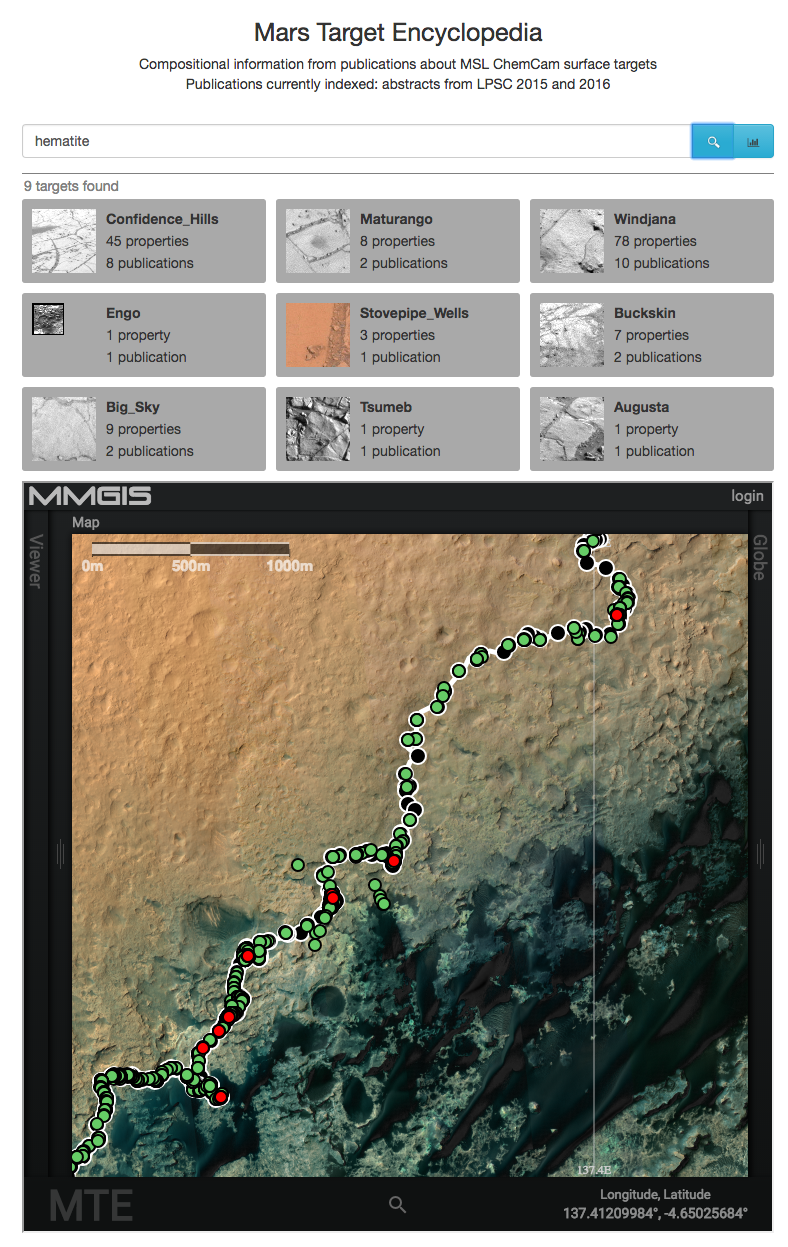
\includegraphics[width=3.25in]{fig/mte-hematite.png}}
\fbox{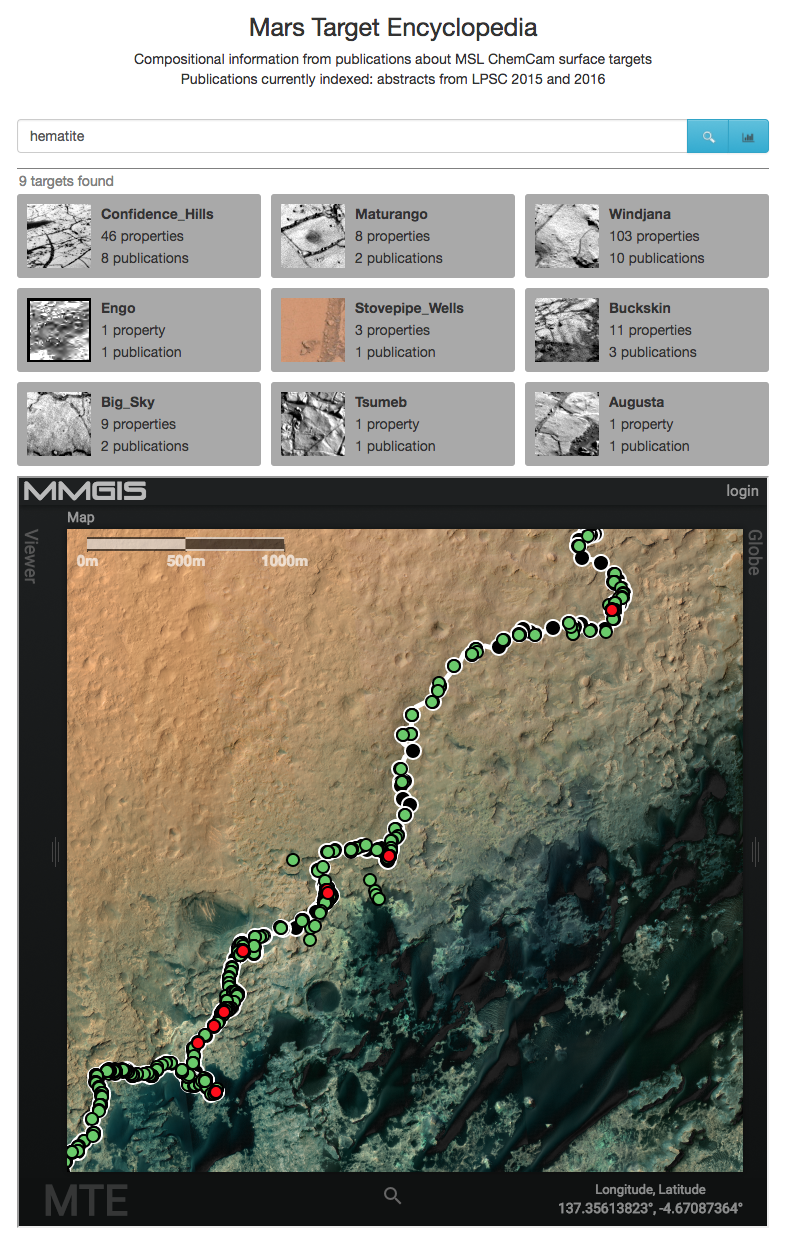
\includegraphics[width=3.25in]{fig/mte-hematite-v2.png}}
\end{center}
\caption{MTE search results for ``hematite.''  Nine results
(individual Mars targets) are returned, and a map displays the
location of each hit, in red.}
\label{fig:mtesearch}
\end{figure}

On the technical side, there are two important limitations to the MTE
content.  First, the current MTE cannot generate overlapping
annotations.  For example, the phrase ``calcium sulfate'' was manually
labeled as ``calcium'' (Element), ``sulfate'' (Mineral), and
``calcium sulfate'' (Mineral).  However, the MTE's NER model only
classifies individual tokens, so it misses the ``calcium sulfate''
phrase. 

Second, the relation extraction module only generates candidate
relation pairs within a sentence.  In this corpus, 32\% of the
manually annotated relations cross sentence boundaries.  Therefore,
the current system cannot yet retrieve those relations.  
% 166 / 463 (35.85%) relations cross sentences.
% lpsc15: 35.85%
% 47 / 210 (22.38%) relations cross sentences.
% lpsc16: 22.38%
% Total: 213/673 = 31.65%
%
% TODO: recalc this number with analyze_brat, restricted to Element
% and Mineral relations
One way to access sentence-crossing relations would be to expanding the
number of candidate entity pairs to include all pairs within a
paragraph.  We plan to evaluate that strategy in future work.

% note that we want to move to a conceptual eval, not per-example
% ``in this doc, does Epworth contain Fluorine?''
%In general, an evaluation strategy that focuses on concepts rather
%than individual relations may better reflect the quality of the
%extracted knowledge.  For example, 

\section{Conclusions and Next Steps}
% and lessons learned

This work lies at the intersection of information extraction, machine
learning, and planetary science.  The MTE uses current IE technology
to provide the first database of Mars target compositional knowledge
as expressed in the scientific literature.  The pipeline is fully
automated, and we can employ web crawlers to seek out new (publicly
accessible) papers as they are published.  We also plan to enable
users to submit their own publications for analysis and augmentation
of the database.

We are in the process of integrating the MTE's content into the MSL
Analyst's Notebook, an interactive web resource for mission scientists
and the interested public~\cite{stein:msl-an13}.  The Analyst's
Notebook allows users to 
browse mission plans, targets discovered, data collected, and
summaries of each mission day on Mars.  The MTE content will enable
the Analyst's Notebook to also connect targets to publications.

The MTE currently contains information about ChemCam targets that was
extracted from three years of papers published at the Lunar and
Planetary Science Conference.  A next logical step is to expand the
MTE to encompass targets identified by other instruments on the
Curiosity (MSL) rover and other missions such as the Mars Exploration
Rovers (Spirit and Opportunity).  In addition, we plan to extend the
MTE to be able to ingest journal papers that have been published by
MSL science team members and the broader community.  This information
will carry more weight because it comes from peer-reviewed sources; users
will be able to restrict their searches to journal papers only, or to
obtain all possible results.

The automatic extraction of knowledge from scientific publications can
benefit many other areas of scientific inquiry.  In addition to
biology and medicine, there are opportunities at the intersection
between fields such as planetary science and astronomy.  For example,
there are currently 3,550 confirmed exoplanets (planets outside our
solar system) as of November 2, 2017~\cite{ipac:exo}.  Hundreds of new
planet candidates are announced each year in new publications.
Desirable properties to extract and store for each planet include its
radius, temperature, period, distance from its host star, and more.
Compositional relationships exist for elements present in the
host star and for constituents in exoplanet atmospheres, with
implications for the possible presence of life on other planets.
In general, extracting information and relationships into a central,
searchable database can help inform new hypotheses and direct future
science investigations.

\section{Acknowledgments}
This research was carried out in part at the Jet Propulsion Laboratory,
California Institute of Technology, under a contract with the National
Aeronautics and Space Administration.  
% TODO:
%{\bf [acks for Ellen?]}
We thank the Multimission Ground System and Services (MGSS)
program and the Mars Science Laboratory project for funding and
enthusiastically supporting this work.
\bibliography{mte}
\bibliographystyle{aaai}
\end{document}

% LocalWords:  tex aaai sty AAAI Thamme Gowda Lanza Lu Riloff Karanjeet Singh
% LocalWords:  CA firstname lastname Del Rey searchable lpsc MTE website PDS IE
% LocalWords:  MSL krallinger tsutsui Alzheimer's GeoDeepDive ISI PDF ChemCam
% LocalWords:  sol NER mte pptx Tika UTF utf py regexp Mg CoreNLP IMA TODO CRF
% LocalWords:  Zr Si Ti REEs alkalies lexico co jSRE Solr Lucene API html ann
% LocalWords:  uniq docs Prec eval CoreNLP's LC GC SL Indiv OpenIE num Fe MTE's
% LocalWords:  rover's recalc doc Epworth acks
